\def \imgpath {"./figures/intro"}
\section{Standard Model of elementary particles}

One paragraph QFT\\
One paragraph description\\
One paragraph successess and drawbacks

\begin{figure}[H]
\includegraphics[width=0.90\textwidth]{\imgpath/SM.pdf}
\caption{Standard model. VALUES NEED TO BE FIXED.}
\end{figure}

\subsection{Quantum Electrodynamics}

One paragraph

\section{Coordinate systems and kinematic observables}

Particles in HEP processes are described by their Lorentz-invariant four-vectors, $\bm{x} = (ct, x, y, z)$ and $\bm{p} = (E/c, p_x, p_y, p_z) = (E/c, \pt, p_z)$. In LHC experiments, the coordinate system is defined such that the $x$-axis points in the direction of the LHC, and the $z$-axis points in the direction of the beam, as shown in Fig.~\ref{fig:intro:coordinates}. In addition to the standard Cartesian coordinates, two observables, $\varphi$ (azimuthal angle) and $\eta$ (pseudorapidity), are used to describe the position and momentum of particles relative to the interaction point, which is located at $x = y = z = 0$. Pseudorapidity is defined as a function of the polar angle $\theta$, where 
\begin{align}
\eta = -\ln(\tan(\theta/2)) \quad .
\end{align}
For high-momentum particles ($p \geq mc$), pseudorapidity is an approximation of the rapidity relative to the beam, given by 
\begin{align}
y = \frac{1}{2} \ln \frac{E + p_z c}{E - p_z c} \quad .
\end{align}
Rapidity is a convenient quantity to use because it transforms additively under Lorentz boosts, unlike velocity. In these coordinates, the following relations hold:
\begin{align}
p_x = |\vec{\pt}| \cos \varphi \, , \quad \
p_y = |\vec{\pt}| \sin \varphi \, , \quad \
p_z = |\vec{p} \,| \sinh \eta \, .
\end{align}

\begin{figure}[H]
\includegraphics[width=0.85\textwidth]{\imgpath/coordinates.pdf}
\caption{Coordinate system of an LHC experiment.}
\label{fig:intro:coordinates}
\end{figure}

\section{Processes involving gluons}

Diagrams, screening(?), divergences

\subsection{Running coupling constant}

One paragraph, one figure

\subsection{Perturbative QCD}

One paragraph

\section{From partons to hadrons}

\subsection{Initial and Final State Radiation}

In quantum field theory, charged particles are surrounded by a cloud of virtual particles, which can be thought of as fluctuations in the particle's field. For example, the electron state can be described as a superposition of the bare electron plus additional massless bosons:
\begin{align}
|\mathrm{e}\rangle_\mathrm{phys} = |\mathrm{e}\rangle + |\mathrm{e}\gamma\rangle + |\mathrm{e}\gamma\gamma\rangle + \ldots
\end{align}
and, at higher orders, pairs of virtual electrons. The fluctuations continuously form and recombine, with their lifetime depending on their energy and momentum. Specifically, the lifetime of a fluctuation with energy $\omega$ and transverse momentum $k_\mathrm{T}$ can be approximated as:
\begin{align}
\tau \approx \frac{\omega}{k_\mathrm{T}} \quad .
\end{align}
This implies that fluctuations with smaller-$k_\mathrm{T}$ live longer.

As illustrated in Fig.~\ref{fig:intro:isrfsrsketch}, the coherent mixed state of the bare charge and the field fluctuations can be disturbed by the presence of an interaction. Intuitively, this interaction can change the energy and momentum of the fluctuations, their formation and recombination, and lead to the emission of radiation in two ways:
\begin{enumerate}
\item a fluctuation is kicked on-shell by the interaction and part of the field continues in its original direction, which leads to Initial State Radiation (ISR);
\item as a result of the field of the scattered particle rearranging itself , which can be a source of Final State Radiation (FSR).
\end{enumerate}

In both of the cases, a larger momentum transfer implies more radiation. \textit{For hard, wide angle emissions, cross sections can be calculated perturbatively at fixed orders}. 

Soft and collinear emissions, however, lead to infra-red divergences ($\propto \frac{1}{\omega}$,$\propto \frac{1}{k_\mathrm{T}^2}$) and thus, need to be factorised away from the amplitudes or the cross sections and then described using resummation techniques. Without any emissions, the probabilities of finding electrons and photons of fractional momentum $x$ with respect to the whole system are:
\begin{align}
f_\mathrm{e} (x) = \delta (1-x) \, , \quad \ f_\gamma(x) = 0 \, ,
\end{align}
When considering the emissions above some scales parametrised by the resolution parameter $Q^2$, these probabilities, however, evolve according to the DGLAP equation:
\begin{align}
\label{eq:intro:dglap}
\frac{\partial}{\partial\ln Q^2}
\begin{pmatrix}
f_e(x, Q^2)\\
f_{\gamma}(x, Q^2)
\end{pmatrix}
&= \frac{\alpha_\mathrm{em}}{2\pi}
\int_x^1 \frac{dz}{z}
\begin{pmatrix}
P_{ee}(z) & P_{e\gamma}(z)\\
P_{\gamma e}(z) & P_{\gamma\gamma}(z)
\end{pmatrix}
\begin{pmatrix}
f_e\left(\frac{x}{z}, Q^2\right)\\
f_{\gamma}\left(\frac{x}{z}, Q^2\right)
\end{pmatrix} \quad ,
\end{align}
where $P_{ij}(z)$ are the splitting probability functions of a particle $i$ emitting a particle $j$.

In QCD, the behaviour is analogous, with $\alpha_\mathrm{em} \rightarrow \alpha_s$, $e\rightarrow q$, and $\gamma \rightarrow g$. 

\begin{figure}[H]
\subfloat[][]{\includegraphics[width=.480\textwidth]{\imgpath/isrfsr1.png}}
\subfloat[][]{\includegraphics[width=.480\textwidth]{\imgpath/isrfsr2.png}}
\caption{Illustration of the field fluctuations and emmisions of radiation in a scattering process.}
\label{fig:intro:isrfsrsketch}
\end{figure}

\subsection{Factorisation theorem}

The evolution equations \ref{eq:intro:dglap} imply that the probabilities of observing emissions with a fractional momentum $x$ depend on the resolution $Q^2$. In QCD, 
\begin{enumerate}
\item when applied to the initial state, they are known as parton distribution functions (PDFs) and determine the probabilities of finding partons\footnote{Partons refer to the valence quarks, sea quarks, and gluons inside hadrons.} in the composite hadronic state. 
\item When applied to the final state, they are called fragmentation functions, and determine the probabilities of measuring fragments of the outgoing particles.
\end{enumerate}

This leads to the factorisation theorem for processes involving collisions of two hadrons, which separates the perturbatively calculable partonic cross section from the non-perturbative partonic evolution and hadronisation. The theorem can be expressed as follows:
\begin{align}
\sigma = f_i^A(x_i,\mu_F)f_j^B(x_j,\mu_F) \otimes \hat{\sigma}_{ij\to n}(\mu_F,\mu_R) \otimes D_{n \to n'} \, .
\end{align}
Here, $i$ and $j$ are the initial partons, $\hat{\sigma}_{ij\to n}$ is the partonic cross section, $D_{n \to n'}$ is the process-specific fragmentation function for evolving the partons $n$ into the particles' final state $n'$, and $\mu_F$ and $\mu_R$ are the factorisation and renormalisation scales, respectively. The factorisation scale, $\mu_F$, determines the scale below which the emissions are absorbed into the PDFs. The theorem is depicted in Fig.~\ref{fig:intro:factorisation}.

\begin{figure}[H]
\includegraphics[width=0.65\textwidth]{\imgpath/factorisation.png}
\caption{Illustration of the factorisation theorem. (NEEDS TO BE REMADE).}
\label{fig:intro:factorisation}
\end{figure}

\subsection{Parton distribution functions}

The PDFs defining the probabilities of finding quarks and gluons in nucleons can be determined experimentally at hadron-electron colliders such as HERA. They are determined from measurements of deep inelastic scatterings in a range of energies and momentum transfers. They are displayed in Fig.~\ref{fig:intro:pdfs} as a function of the fractional momentum $x$ (also called Bj\"orken $x$). 

According to collider kinematics, $x \propto \frac{1}{\sqrt{s}e^y}$, therefore, the partonic composition of ultra-relativistic hadrons is dominated by gluons. Following unitarity principles and BK evolution equation, it is expected that gluons start recombining and the gluonic content saturates as $x\rightarrow0$. This is actively reseached, however, not directly measured yet. Additionally, it should be noted that in ultra-relativistic heavy nuclei, the partons are modified in the contracted nuclear environment and the PDFs are referred to as nPDFs.

\begin{figure}[H]
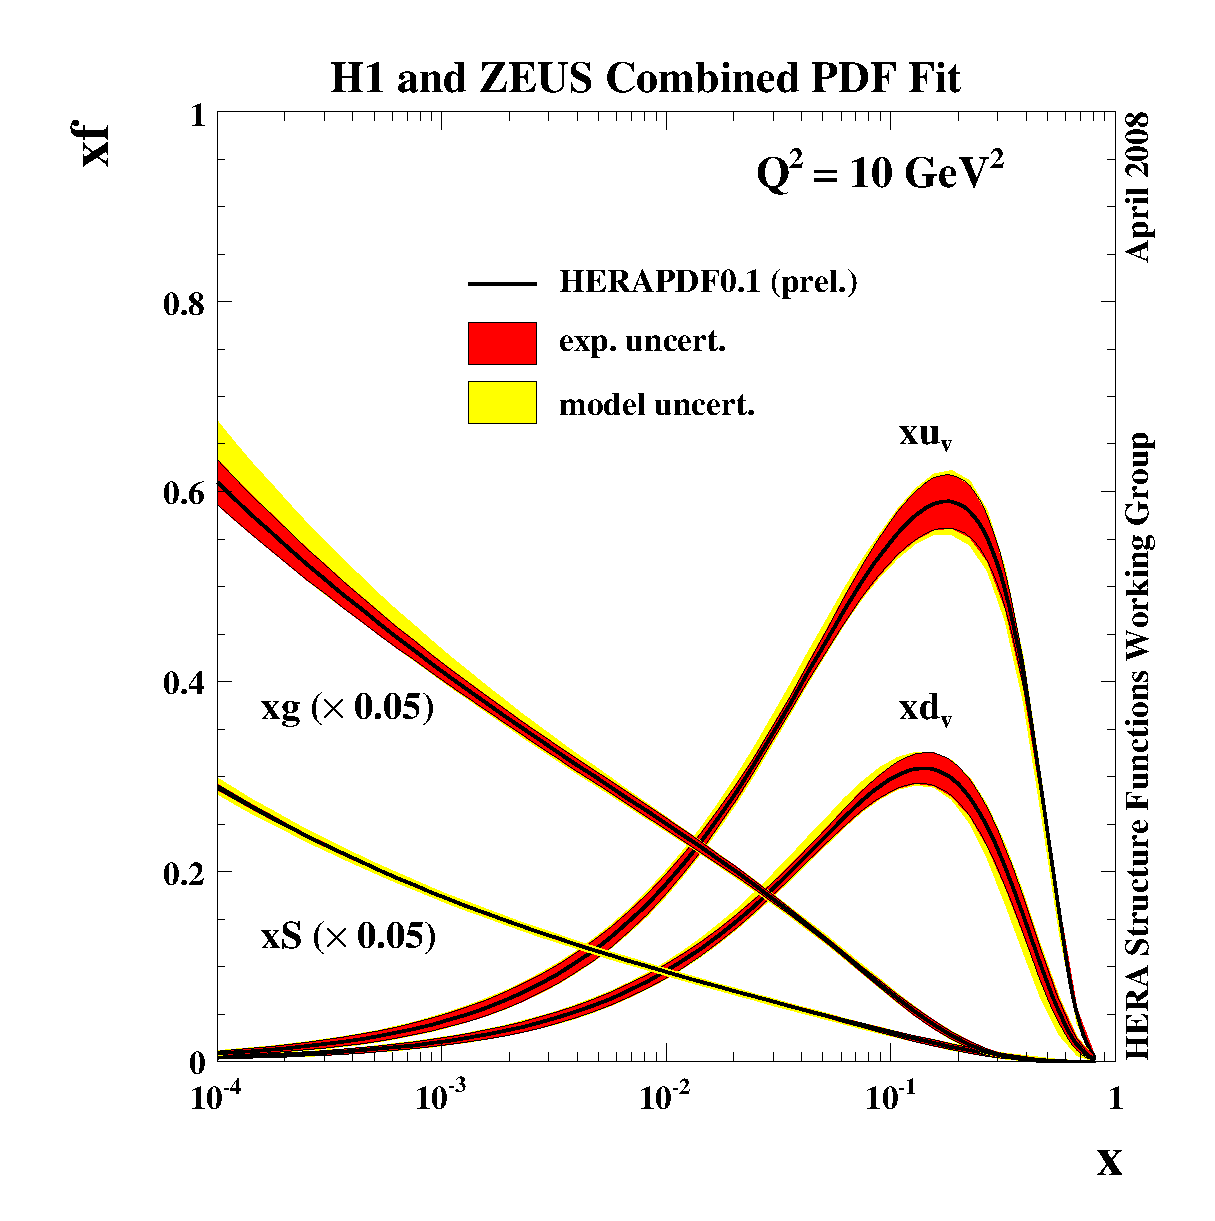
\includegraphics[width=0.4\textwidth]{\imgpath/pdf.eps}
\caption{Parton distribution functions determined at HERA. TBA}
\label{fig:intro:pdfs}
\end{figure}

\subsection{Parton fragmentation and the Lund string}

After the scattering process, the produced partons continue to fragment by emitting more partons in a process called the parton shower. Since the coupling strength in QCD increases with decreasing the energy scale of the splitting, this leads to the production of many soft, collimated emissions known as jets. The partonic evolution continues until the virtuality of the partons reaches the hadronization scale ($\approx \Lambda_\mathrm{QCD}$). There are multiple frameworks within QCD to describe the evolution of partons into their final state, such as using the DGLAP equations or the so-called dipole formalism.

Once the partonic final state is reached, the partons hadronise into the observable mesons and baryons. The hadronisation process is not calculable in QCD and requires phenomenological models to describe it. One such model is the Lund String model, which describes hadronisation as the breaking of a color string between the quarks in the final state. In this model, the energy stored in the color string is converted into the mass of new hadrons.

According to confinement, hadronisation should involve at least two partons with complementary colours. In QCD, the $q\bar{q}$ potential takes the shape of
\begin{align}
V_{q\bar{q}} \approx - \frac{4}{3}\frac{\alpha_s \hbar c}{r} + \kappa r \quad ,
\end{align}
where $\kappa$ is a paramater with value around $1 \mathrm{GeV} /\mathrm{fm}$. In the non-perturbative regime (long distances), the potential is dominated by the linear part, which is reminiscent of a system bound by a string with tension $\kappa$. This is taken advantage of by the Lund string model -- a $q$ and $\bar{q}$ pair separated by distance $\Delta x$ is bound by a color field (string) with energy $\kappa \Delta x$. 

If the $q$ and $\bar{q}$ continue separating as a result of the scattering, the energy stored in the color field increases. At some point, it can become energetically favourable to produce a new $q\bar{q}$ pair out of vacuum, which is a quantum mechanics tunnelling phenomenon characterised by the probability:
\begin{align}
\frac{\mathrm{d}P}{\mathrm{d}m_\mathrm{T}} \propto \exp \left( -\frac{\pi m_\mathrm{T}^2}{\kappa} \right) \quad ,
\label{eq:intro:tunnel}
\end{align}
where $m_\mathrm{T}$ is the transverse mass of the produced quarks. Otherwise, the $q\bar{q}$ system starts contracting and oscillates with a period $T = 2 E_\mathrm{kin}/\kappa$, where $E_\mathrm{kin}$ is its maximum kinetic energy. The produced $q$ and $\bar{q}$ then connect by new color fields to the original pair. This process repeats itself result in cascade of many $q\bar{q}$ pair connected by many color strings. In this descriptions, baryons can also be created by double tunnelling of a $qq\bar{qq}$ pair. The process is illustrated in Fig.~\ref{eq:intro:lundstring}.

\begin{figure}[H]
\subfloat[][]{\includegraphics[width=.330\textwidth]{\imgpath/tubelike.png}}
\subfloat[][]{\includegraphics[width=.330\textwidth]{\imgpath/lundstring.png}}
\subfloat[][]{\includegraphics[width=.330\textwidth]{\imgpath/lundgluon.png}}
\caption{Illustration of the color field between two quarks and its simplified representation with a string. Illustration of the string splitting by producing new $q\bar{q}$ in the $t-z$ plane. Illustration of the treatment of gluons in the Lund string model.}
\label{fig:intro:lundstring}
\end{figure}

Equation \ref{eq:intro:tunnel} also implies that production of strange quarks is suppressed by a factor of 
\begin{align}
\rho = \exp \left( -\frac{\pi (m^2_s - m^2_{u,d})}{\kappa} \right) \quad .
\end{align}
This parameter is typically tuned to data, as substituting constituent ($m_s \approx \gevcc{0.5}$, $m_{u,d} \approx \gevcc{0.33}$) versus current masses ($m_s \approx \gevcc{0.1}$, $m_{u,d} \approx 0$) leads to considerable differences underestimating and overestimating data, respectively.

For a $q\bar{q}g$ system, in this model, the gluon connects to the quark and antiquark and is effectively treated as a ``kink" on the color field, adding energy and momentum to the $q\bar{q}$ string (stretching it in its direction), as visualised in Fig.~\ref{eq:intro:lundstring}.

It should be noted that in the paradigm of AA collisions, hadron production can be alternatively modelled by hadronisation at the QGP's phase boundary by \textit{coalescing} free quarks.
%CooperFrye freezeout

%%!!!!TBA a sentence about the actual hadronisation.

\section{Multiple partonic interactions}

Results from $\mathrm{Sp\bar{p}S}$ in the 1980s sparked motivations for considering interactions of multiple partons between the two composite protons. For example, the AFS experiment observed an abundance of 4-jet events, displayed in Fig.~\ref{fig:intro:afs4jet}, that could not be explained by calculations considering a double gluon bremststrahlung from a single partonic scattering\cite{afs-4jet}. Furthermore, UA5 measurements studying energy dependence of multiplicity distributions P(\Nch) from  revealed a significant broadening when increasing $\sqrt{s}$, and saw the so-called KNO scaling\cite{kno-scaling}, where P(\Nch)/\meanNch remains constant, which was not reproducible in the context of \Nch being produced from a single string\cite{ua5-broadening}. This further suggested at the presence of multiple production sources.

\begin{figure}[H]
\subfloat[][]{\includegraphics[width=.520\textwidth]{\imgpath/afs4jet.png}} 
\subfloat[][]{\includegraphics[width=.380\textwidth]{\imgpath/sigmampi.pdf}}
\caption{TBA.}
\label{fig:intro:afs4jet}
\end{figure}

These findings prompted further development of Regge theory and approaches that incorporated multiple pomerons, which were successful in describing the \Nch distributions. However, this approach is fully decoupled from descriptions of the perturbative primary scattering. Subsequently, much of the phenomenology related to multiple partonic interactions was developed within the framework of the Pythia MC event generator, which is discussed individually in Section X. However, nowadays, the relevance of the concept of MPIs in hadronic collisions extends beyond this generator. A scattering with double partonic interactions is illustrated in Fig.~\ref{fig:intro:dps}.

\begin{figure}[H]
\includegraphics[height=7em]{\imgpath/dps.png}
\caption{TBA.}
\label{fig:intro:dps}
\end{figure}

In the Pythia approach, MPI are treated as additional perturbative scatterings. In QCD, the $2\to2$ cross section (dominated by the gluon exchange t-channel) diverges as $\propto \alpha^2_S(k_{\perp}^2)/k_{\perp}^4$, so a cutoff parameter $k_{\perp/\mathrm{min}}$ must be introduced, and using (\ref{fig:intro:factorization}) leads to:
\begin{align}
\frac{d\sigma}{dk_{\perp}^2} &= \sum_{ij}\int dx_1 dx_2 f_i(x_1,\mu_F^2)f_j(x_2,\mu_F^2) \frac{d\hat{\sigma}^H_{ij}}{dk_{\perp}^2} \, , \\
\sigma_{\text{int}}(k_{\perp\text{min}}) &= \int_{k_{\perp\text{min}}^2}^{s/4} \frac{d\sigma}{dk_{\perp}^2}dk_{\perp}^2 \, .
\end{align}
The choice of cutoff can be tuned to experimental data, and for the $\mathrm{Sp\bar{p}S}$ energy of \sppg{630}, a value of around \gevc{1.6} was typical. The dependence of this parton-parton scattering cross section is shown in Fig.~\ref{fig:intro:afs4jet}.

The total pp cross-section is given by
\begin{align}
\sigma_{\mathrm{pp}} &= \sigma_{\mathrm{elastic}} + \sigma_{\mathrm{single \, dif.}} + \sigma_{\mathrm{double \, dif.}} + \sigma_{\mathrm{non-dif.}} \quad , 
\end{align}
where the inelastic cross sections corresponds to approximately 60\% of the total. The mean number of MPIs, \meannmpi, can be estimated using:
\begin{align}
\meannmpi (k_{\perp,\mathrm{min}}) = \frac{\sigma_{\mathrm{int}}(k_{\perp,\mathrm{min}})}{\sigma_{\mathrm{inel}}}
\end{align}

However, the actual treatment is more complex and involves considerations of other parameters such as $k_\perp^0$ to account for the confinement nature of partons, modifications of multiparton PDFs, energy-momentum conservation, and the intertwinedness of partonic evolutions.



In summary, MPIs represent several subcollisions that take place in an average pp collision with \pt scales of a few GeV. They are colour-connected to the beam remnants, which in the Lund model are represented by strings. Since a string with $\kappa = 1 \mathrm{GeV} /\mathrm{fm}$ yields, as a rule of thumb, approximately one hadron per unit rapidity, and the average pp collision at the LHC at \sppt{13} has $\langle \dndy \rangle \approx 6$, the typical number of partonic interactions is around six.

Finally, the observation of QGP-like phenomena in pp collisions at the LHC has renewed interest in MPI phenomenology, as discussed in the following chapter. Such observations do not contradict the concept of MPIs; rather, they suggest the possibility of incorporating collective behavior among the MPIs, such as interactions between strings, local modifications of string tensions, or, alternatively, the formation of a multipartonic state with QGP-like properties.

\subsection{Color reconnection}

The incorporation of MPIs improved the description of the \Nch distributions and their dependence on $\sqrt{n}$. However, there were also observations of $\meanpt(\Nch)$ increasing as a function of \Nch, which could not be explained. More MPIs lead to more strings, which in turn leads to the production of more particles, but the \pt is mostly unaffected. This would predict a weaker dependence of \meanpt on \Nch, contrary to the data. The issue was resolved by implementing a possible color reconnection mechanism, which rearranges the color fields between partons.

TBA Insert diagrams of the processes!

One can envision the following process:
\begin{align*}
e^+ e^- \rightarrow W^+ W^- \rightarrow q_1\bar{q}_2 q_3\bar{q}_4  .
\end{align*}
In this scenario, a color reconnection mechanism could rearrange the colour-connected $q_1\bar{q}_2$ and $q_3\bar{q}_4$ into $q_1\bar{q}_4$ and $q_3\bar{q}_2$ if it were energetically favourable, depending on the phase-space configurations. Measurements at LEP of this process have indeed shown that such final-state corrections must be taken into account to explain the data on $W$ masses and widths. They also reported that the reconnection probabilities for such events are on the order of $50\%$, further indicating that colour reconnection is an important factor to consider.

Pythia implements CR by minimizing the total length of strings in the system, analogous to minimising potential energy. This mechanism, illustrated in Fig.~\ref{fig:intro:cr}, explains the rising trend of $\meanpt(\Nch)$: shorter strings imply fewer hadrons to split the transverse boost across, and the more MPI, the bigger this effect. Moreover, CR also helped describe the absolute value of \meanpt. With this approach, no further modifications of fragmentation parameters were necessary, in line with the concept of jet universality. However, it should be noted that there are various CR implementations and all rely on parameters obtained from tuning to data.

\begin{figure}[H]
\includegraphics[height=7em]{\imgpath/cr.png}
\caption{a) In a hard parton subcollision, the outgoing gluons are connected to the beam remnants through colour. Additional gluon kinks may occur through initial state radiation, which are ordered by rapidity. (b) A second hard scattering should theoretically result in two new strings connected to the remnants. (c) In order to minimise the total string length, gluons are colour reconnected.}
\label{fig:intro:cr}
\end{figure}

It is also worth noting that the \pt boost acquired through color reconnection may depend on mass and whether a hadron is a baryon or meson, which somewhat mimics the hydrodynamic signatures of collective flow observed in AA collisions.

\section{Underlying event}

The underlying event (UE) in high-energy collisions refers to the additional hadronic activity that accompanies the primary hard scattering process, but is not directly related to it. This includes the fragmentation products of the beam remnants, ISR and FSR, as well as the effects of the previously discussed MPIs. The UE is typically characterized by the distribution of softer particles around and far outside of the hard process.

It is important to note that the UE is different from the MB production, as it is biased by the presence of hard scattering. Additionally, the magnitude of the UE can fluctuate from event to event.

TBA Maybe some illustration/plot

\section{Lattice QCD}

One paragraph

\section{QCD phase diagram}

One paragraph, figure

\subsection{Phase transition}

One paragraph, bag model derivation of $T$

\subsection{Chiral symmetry restoration}

One paragraph, figure

\section{Implications of high-activity QCD research}

One paragraph